%------------------------------------------------------------------------
%Editar Diplomado
\hypertarget{cv:eliminarModulo}{\section{Eliminar Módulo}} \label{sec:eliminarModulo}

	Esta funcionalidad le permitirá eliminar un módulo innecesario o incorrecto. Para eliminar un módulo es necesario que no tenga pantallas o casos de uso asociados a el.

		\subsection{Procedimiento}

			%Pasos de procedimiento
			\begin{enumerate}
	
			\item Oprima el botón \IUBotonEliminar{} de un registro existente de la pantalla \ref{fig:GestionarModulos} ''Gestionar Módulos''.
	
			\item Se mostrará el mensaje \ref{fig:confirmaEliminaModulo} sobre la pantalla \ref{fig:GestionarModulos} ''Gestionar Módulos''.
			
			%Pantalla
			\begin{figure}[htbp!]
				\begin{center}
					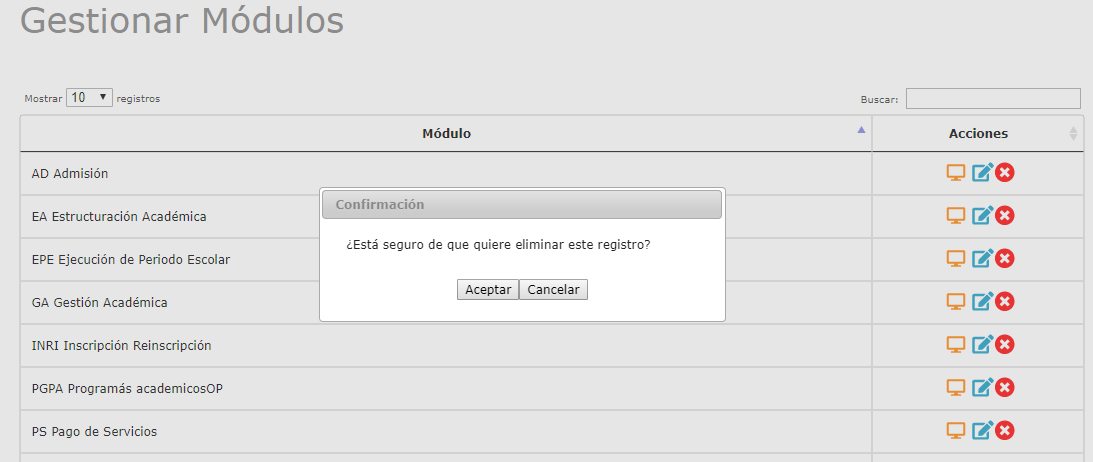
\includegraphics[scale=0.6]{roles/lider/modulos/pantallas/IU5-3MSG10}
					\caption{MSG de Confirmación}
					\label{fig:confirmaEliminaModulo}
				\end{center}
			\end{figure}
						
			\item Oprima el botón \IUAceptar.
			
			\item Se mostrará el mensaje \ref{fig:moduloEliminado}  (Pendiente) en la pantalla \ref{fig:GestionarModulos} ''Gestionar Módulos''.
			
			\begin{figure}[htbp!]
				\begin{center}
					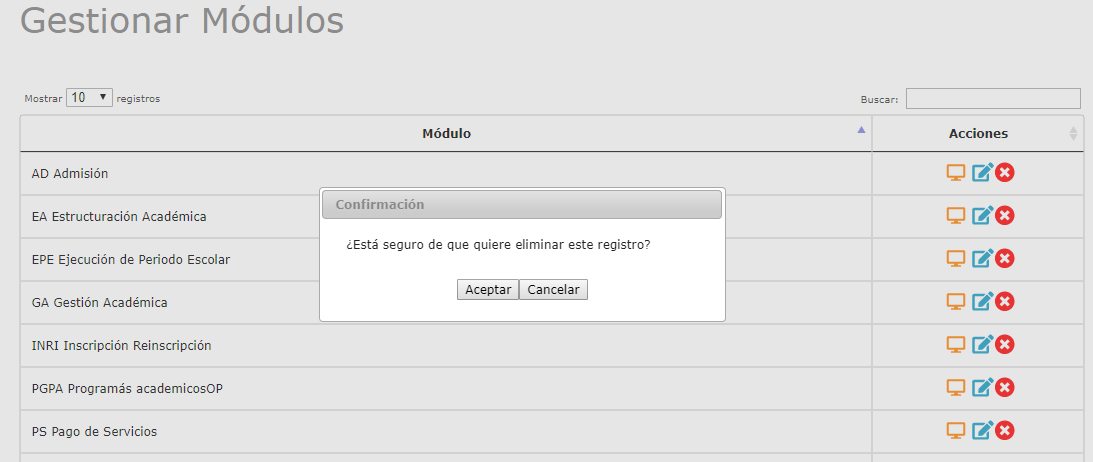
\includegraphics[scale=0.6]{roles/lider/modulos/pantallas/IU5-3MSG10}
					\caption{MSG: Módulo Eliminado}
					\label{fig:moduloEliminado}
				\end{center}
			\end{figure}
			\end{enumerate}